% Auto-generated by generate_report.py — do not edit manually
% Preamble mirrors oxengthesis.cls so figures match the body text:
% Carlito as main font, Latin Modern Math via unicode-math.
\documentclass[border=6pt]{standalone}
\usepackage{fontspec}
\setmainfont{Carlito}
\usepackage{unicode-math}
\setmathfont{Latin Modern Math}
\usepackage{pgfplots}
\pgfplotsset{compat=1.18}
\usepgfplotslibrary{groupplots}
\usetikzlibrary{patterns,positioning}
\begin{document}
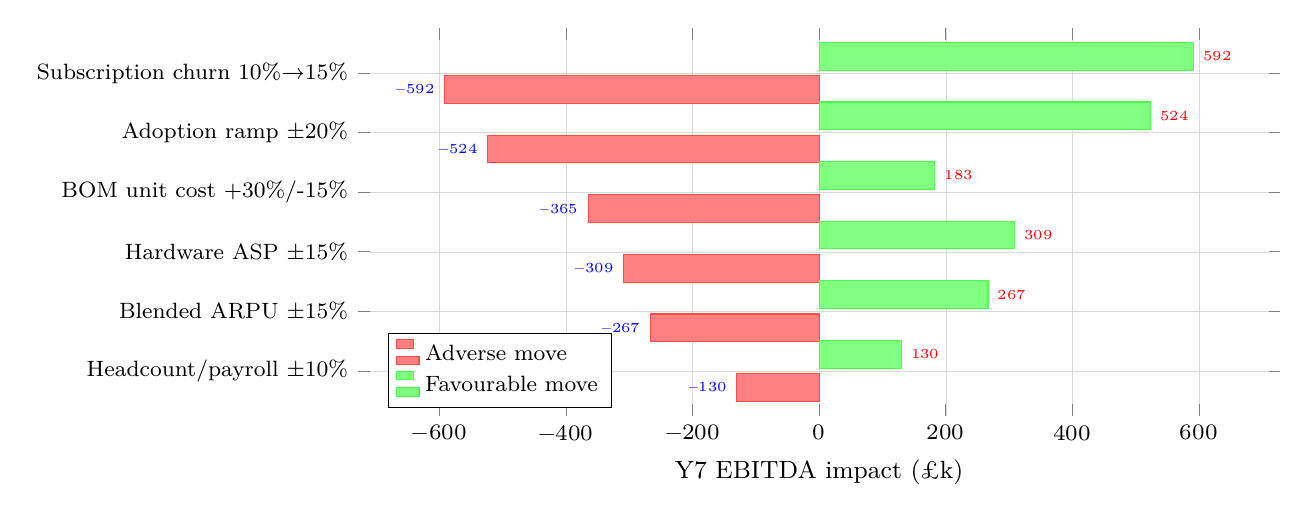
\begin{tikzpicture}
    \begin{axis}[
        width=13cm,
        height=6.5cm,
        xbar,
        bar width=10pt,
        xlabel={Y7 EBITDA impact (\pounds k)},
        symbolic y coords={{Headcount/payroll ±10\%},{Blended ARPU ±15\%},{Hardware ASP ±15\%},{BOM unit cost +30\%/-15\%},{Adoption ramp ±20\%},{Subscription churn 10\%→15\%}},
        ytick=data,
        y axis line style={opacity=0},
        enlarge y limits=0.15,
        nodes near coords,
        nodes near coords style={font=\tiny},
        nodes near coords align={horizontal},
        grid=major,
        grid style={line width=.1pt, draw=gray!30},
        legend style={
            at={(0.02,0.02)}, anchor=south west, font=\footnotesize,
            legend cell align={left},
        },
        tick label style={font=\footnotesize},
        label style={font=\small},
    ]
    \addplot+[xbar,fill=red!50,draw=red!70] coordinates {(-130,{Headcount/payroll ±10\%}) (-267,{Blended ARPU ±15\%}) (-309,{Hardware ASP ±15\%}) (-365,{BOM unit cost +30\%/-15\%}) (-524,{Adoption ramp ±20\%}) (-592,{Subscription churn 10\%→15\%})};
    \addplot+[xbar,fill=green!50,draw=green!70] coordinates {(130,{Headcount/payroll ±10\%}) (267,{Blended ARPU ±15\%}) (309,{Hardware ASP ±15\%}) (183,{BOM unit cost +30\%/-15\%}) (524,{Adoption ramp ±20\%}) (592,{Subscription churn 10\%→15\%})};
    \legend{Adverse move, Favourable move}
    \end{axis}
\end{tikzpicture}

\end{document}
